\textbf{A few words on epigenomic data}

We illustrate the performances of DEScan2 using a dataset \cite{Su2017} describing adult mouse dentate granule neurons in vivo before and after synchronous neuronal activation using Atac-Seq and RNA-Seq technologies (see sections \ref{sec:atacseq} and \ref{sec:rnaseq}).

This dataset is organized in 62 samples of Atac-Seq and RNA-Seq, sampling them at different time points, with four replicates for time point.
Of this samples we chose to compare the differences at the first two stages, time 0 (E0) and After 1 hour of neuronal induction (E1), in order to show a possible Atac-Sec workflow for Differential Enrichment, and how to integrate this type of data with RNA-Seq data.

\begin{figure}[H]
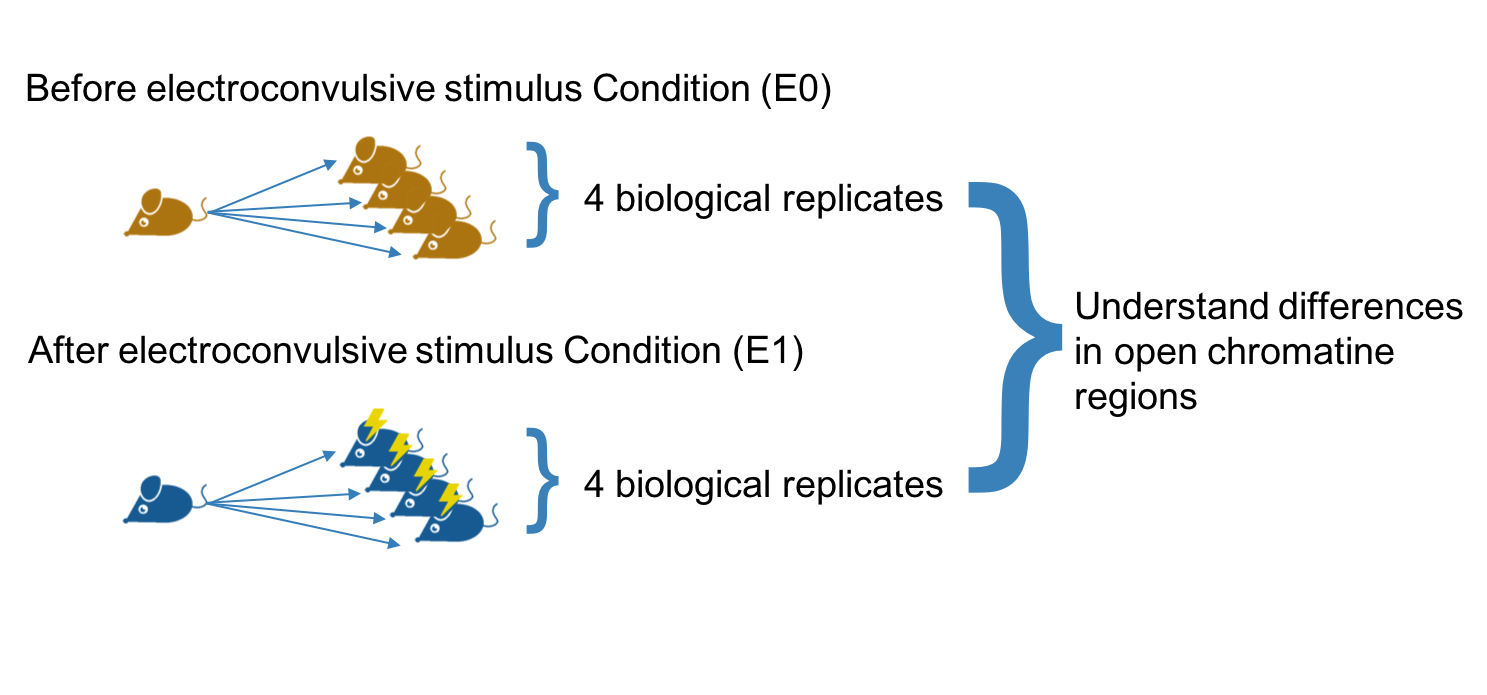
\includegraphics[width=\textwidth,height=\textheight,keepaspectratio]{img/descan2/dataset.png}
\caption{An illustration of our extraction of the \cite{Su2017} dataset.}
\label{fig:atacdataset}
\centering
\end{figure}

We downloaded the data from the \textit{GEO} database \cite{Edgar2002, Barrett2013} with accession number GSE82015\footnote{\url{https://www.ncbi.nlm.nih.gov/geo/query/acc.cgi?acc=GSE82015}} and mapped raw data using \textit{STAR} \cite{Dobin2013} with default parameter on Mus Musculus Genome ver.10 (mm10).

In order to detect the open chromatin regions we run our peak caller, cutting the genome in bins of 50bp and using running windows of minimum 50bp and maximum 1000bp. In such a way we are able to detect not just broad peak, but also smaller peaks.

To be confident with our results we compared the DEScan2 detected peaks on two genes (Arc and Gabrr1) with the same genes validated in \cite{Su2017}.
Lower part of figure \ref{fig:peaksdescan} shows the detected and validated regions (in blue and red) resulting differentially enriched between the E0 (in pink) and E1 (in green) samples, while the upper part shows DEScan2 peaks (in blue), which is able to catch the same regions of the published ones, but also (gold circles) to be more careful in the detection of smaller peaks.

\begin{figure}[H]
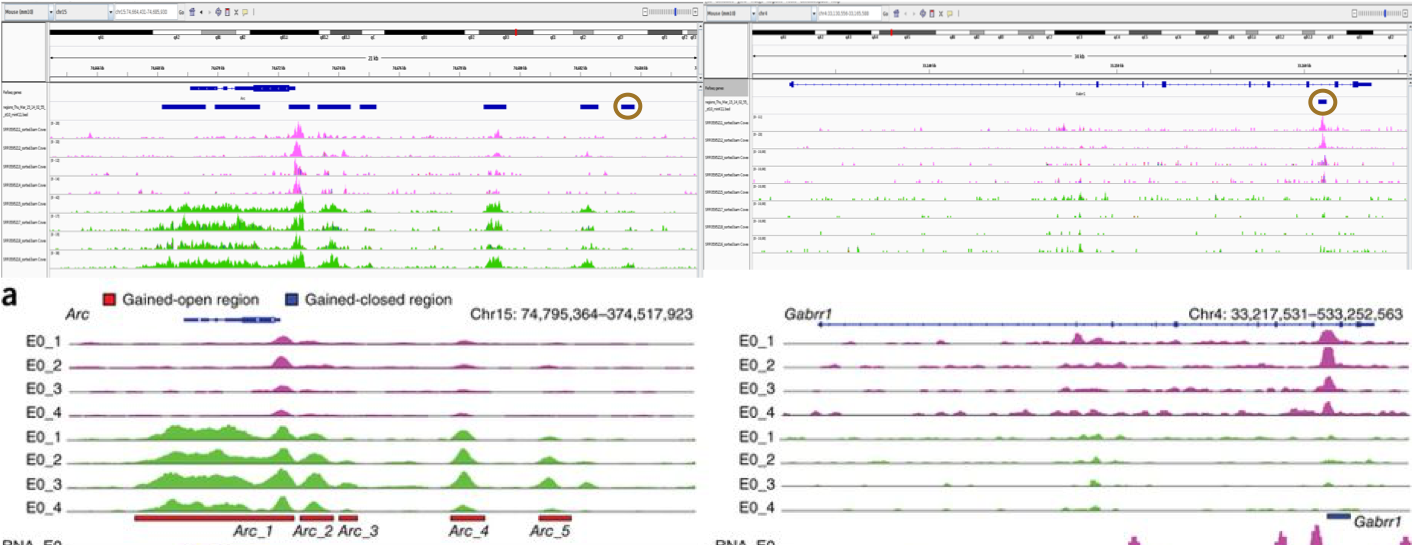
\includegraphics[width=\textwidth,height=\textheight,keepaspectratio]{img/descan2/peaks.png}
\caption{A comparison of DEScan2 detected peaks with validated peaks in article \cite{Su2017}.}
\label{fig:peaksdescan}
\centering
\end{figure}
